\chapter{Daganatos sejtek modellezése}
A tumorkeletkezés leggyakoribb oka az emberi génállományban található, a növekedést szabályozó gén aktiválódása. Ez vezet a szövetregeneráció során rendellenes utódsejtek képzéséhez, amelyek az egészséges szövetbe betörve versenyeznek az erőforrásokért. Többféle daganatos sejt is kialakulhat, mind különbözőképp hatva a környezetére, és így egy olyan változatosság alakulhat ki amely segíti az elszaporodást, egyre erősebben képes ellenállni a kezeléseknek. A játékelmélet egy lehetséges eszköz lehet az ezek közötti versengés modellezésére.

\begin{figure}[h!]
	\centering
	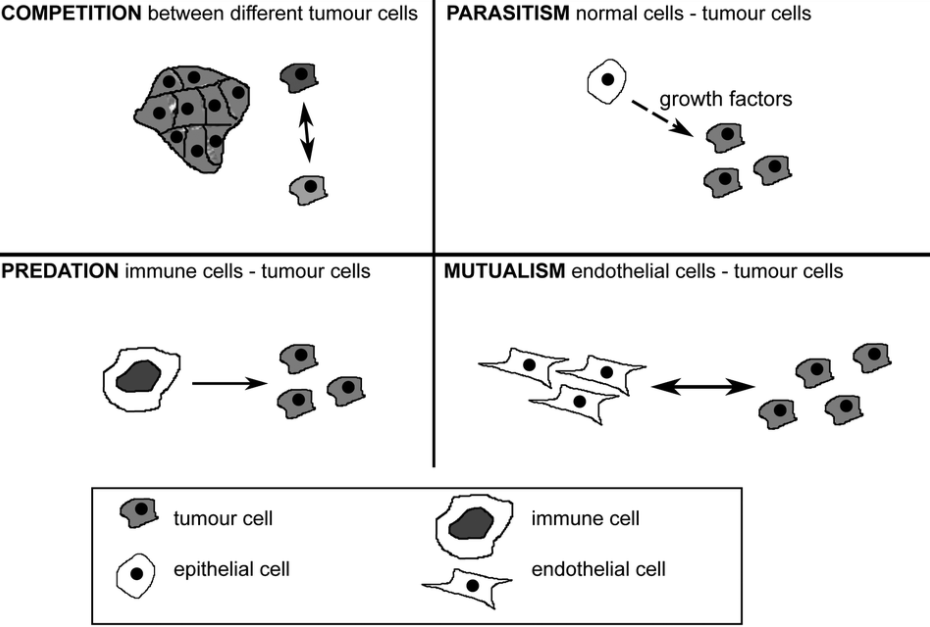
\includegraphics[width=90mm]{images/models}
	\vspace*{2mm}
	\caption{Daganatos sejtek közötti verseny típusok}
	\label{fig:cancerModels}
\end{figure}

A evolúciós játékelméleti modellek segítségével többféleképpen is megközelíthető a probléma. Játékosok lehetnek csak a daganatos sejtek és a játékot az erőforrásokért folytatott \textit{verseny} jelenti. Ez a verseny átalakulhat \textit{parazitizmussá} ha a bizonyos növekedési faktorokat termelő egészséges sejteket tekintjük az egyik félnek, és az ezt kihasználó daganatos sejteket a másiknak. Az immunsejtek játszhatják a \textit{ragadozó} szerepét de felléphet \textit{mutualizmus} is például az erek belső rétegének sejtjei és a daganatos sejtek között (\ref{fig:cancerModels}). 

\section{Közjó játék (Public goods game)}
A daganatos sejtek több jellegzetességének kialakulásában fontos szerepet játszanak az általuk termelt növekedési faktorok és jelzőmolekulák. Ezek segítenek többek között abban, hogy a rákos sejtek a saját növekedésüket ösztönözzék, hogy képesek legyenek kijátszani a szervezet védekezési rendszerét és hogy szétterjedjenek távoli szövetekbe (metasztázis). Mivel ezek az anyagok kikerülnek a sejtek közötti térbe, nem csak az őket termelő sejtekre vannak hatással, hanem az ezeket körülvevőkre is. Így a növekedési faktor felfogható mint egy "közös jó" (\textit{public good}). Az evolúciós játékelmélet megfelelő keretet biztosít, mivel nem feltételez racionális viselkedést és egy stratégia sikerességét megadja a populáción belüli gyakorisága \cite{archetti2016cooperation}.

\section{A játék felépítése}
\subsection{Voronoi diagram}
Az általunk vizsgált modell eltér a megszokottól abban, hogy a sejtek ábrázolására Voronoi hálózatokat használ. Térbeli játékok esetén általában szabályos pontrácsokkal vagy skála-független hálózatokkal dolgoznak. Míg az előbbi figyelmen kívül hagyja a kapcsolatok sokféleségét, az utóbbi nem megfelelő, ha az egyedek egy síkban helyezkednek el \cite{archetti2016cooperation}.

Legyen egy \textit{X} metrikus térben \textit{d} a távolságfüggvény, \textit{K} indexhalmaz, \(\{P_k\}_{k \in K}\) pedig \textit{X} nemüres résztereinek listája. A \(P_k\)-hoz tartozó \(R_k\) Voronoi cella a \(P_k\)-hoz legközelebbi pontok halmaza: 
\begin{equation}
R_k = \{x \in X | d(x,P_k) \leq d(x,P_j), \forall j \neq k\}
\end{equation}
ahol \(d(x,A) = inf\{d(x,a)|a \in A\}\) \textit{x} pont távolságát jelöli \textit{A} résztértől. Egy Voronoi diagram Voronoi cellák rendezett listája
  

\subsection{A játék szereplői és a stratégiák}
A játékban résztvevő sejtek két stratégia közül választhatnak: \textit{kooperálnak}, azaz termelnek növekedési faktorokat, vagy \textit{defektálnak}, azaz nem vesznek részt a faktorok termelésében. A stratégiák \textit{nyereségének (payoff)} kiszámítására a következő képletet használtuk: \(p = b(j) - c\) ahol a \textit{c} a növekedési faktor előállításának költsége, \textit{j} a csoportban résztvevő kooperatív sejtek száma és
\begin{equation}
b(j) = [V(j) - V(0)]/[V(n) - V(0)]
\end{equation}
a
\begin{equation} \label{eq:payoffGradient}
V(j) = 1/[1 + e^{(-s(j-k)/n)}]
\end{equation}
függvény normalizált alakja. A \textit{k} befolyásolja az áthajlási pont helyét, az \textit{s} irányítja a függvény meredekségét az áthajlási pontban. A vizsgált csoport méretét az \textit{n} jelöli. 

A kezdeti populációban véletlenszerűen elhelyezünk defektáló sejteket (alapértelmezetten az arányuk 0.05). Ezután minden körben véletlenszerűen kiválasztunk egy sejtet és annak egy szomszédját és megvizsgáljuk a nyereségeket. Amennyiben a szomszéd stratégiája kifizetődőbb, a kiválasztott sejt átveszi azt. Minden kör végén aktualizáljuk a nyereségeket, hiszen a stratégiák változtatásával változik a \textit{j} értéke és azzal a nyereségek is (aszinkron módon számolunk). 

\subsection{Diffúziós távolság}
A dolgozatunkban vizsgált modell másik újítása, hogy nem csak az elsőfokú szomszédokat veszi figyelembe, hanem egy bizonyos diffúziós távolságon belül található összes sejtet. A szomszédos termelő sejtek befolyásának súlyozására egy diffúziós gradienst vezetünk be. 
\begin{equation}
G(i) = [g(i) - g(0)]/[g(D) - g(0)] 
\end{equation}
és
\begin{equation} \label{eq:diffGradient}
g(i) = 1/[1 + e^{(-z(i-d)/D)}]
\end{equation}
függvények segítségével kiszámolhatjuk az \textit{i} távolságra található kooperatív sejtek befolyásának mértékét. Így a termelők száma nem a fent említett \textit{j} lesz, hanem a \textit{G}-vel kiszámított súlyozott összeg. A képletben szereplő \textit{d} és \textit{D} a diffúziós gradiens alakját határozzák meg, a \textit{z} a gradiens meredekségét az áthajlási pontban \cite{archetti2016cooperation}. Ezzel a modellünk jobban visszaadja azt ami a valóságban történik, hisz a sejtek nem csak a közvetlen szomszédokkal vannak kölcsönhatásban, hanem távolabbiakkal is.

\section{Osztódás}
Kezdeti szimulációink során nem vettük figyelembe azt, hogy a sejtek életük során szaporodni, azaz osztódni is szoktak, ezért mint saját újítás beépítettünk a modellbe egy osztódási lehetőséget is. 

A legtöbbet használt modell, mely elég közel áll a természethez, az a Gompertz modell \cite{wiki:gompertz}, amely leírja a tumor méretének időbeli változását a következő képlettel:
\begin{equation}
	n_t = K \bigg(\frac{n_0}{K} \bigg) ^ {e^{(- \alpha t)}},
\end{equation}
ahol $n_t$ a populáció mérete a $t$ időpillanatban, $n_0$ a populáció kezdeti mérete, $K$ az elérhető maximális mérete a tumornak, míg az $\alpha$ egy konstans, mely a sejtek burjánzási képességével áll összefüggésben. Ez a modell nem csak egy valósághoz közeli képet ad, de azt is biztosítja, hogy a sejtek száma nem nő túl nagyra, mert az a szimulációs rész során komoly lassuláshoz vezetne. 

A játék során használt modellbe könnyen beépíthető, viszont nem veszi figyelembe azt, hogy éppen milyen típusú sejt (kooperáló/defektáló) osztódik. Ez nem azt jelenti, hogy az eredmény amit így kapunk nem elég pontos, hanem azt, hogy nem minden esetben jó ez a megközelítés. Az is megtörténhet, hogy a defektáló sejtek gyorsabban terjednek mint a kooperálók és így egy hibás képet kapunk a játékról.